\documentclass[article]{IEEEtran}
\IEEEoverridecommandlockouts

\usepackage{cite}
\usepackage{amsmath,amssymb,amsfonts}
\usepackage{algorithmic}
\usepackage{graphicx}
\usepackage{textcomp}
\usepackage{xcolor}
\usepackage{listings}

\def\BibTeX{{\rm B\kern-.05em{\sc i\kern-.025em b}\kern-.08em
    T\kern-.1667em\lower.7ex\hbox{E}\kern-.125emX}}
\begin{document}




\definecolor{Base}{HTML}{F0F0F0}
\lstset{backgroundcolor=\color{Base}}
\title{Electronics Laboratory 01\\
\large UADY Faculty of Engenieering}
\author{Sebastian Alejandro Tuyu Piñeiro}

\maketitle

\begin{abstract}
Review of basic electronic components and theory of semiconductors.
\end{abstract}

\section*{Introduction}

Ohm's Law describes the behavior of current in electric circuits, first equation shows us how the voltage inside a resistor is proportional to the current I. \\
\begin{equation}
    V = R \cdot I
\end{equation}

\textbf{Where $R$ is the resistor value.}

When the currents flow inside a resistor, there is an energy dissipation that is described by the following equation: 

\begin{equation}
    P = I^2 \cdot R
\end{equation}

\section*{1st Part. Parallel-Series Circuits
}
\begin{center}
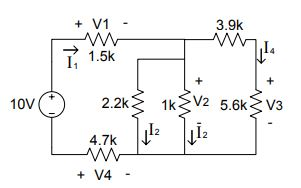
\includegraphics[scale=0.95]{fig1.JPG}

Figure 1. Circuit for exercise 1.
\end{center}

\section*{Calculating the color-code in each resistor}
In every resistor, there are from 4 to 6 color bands indicating the value of the resistor, using that color-format, each resistor would look like:
\begin{itemize}
    \item Resistor 1:
Value, value, value, value
    \item Resistor 2:
Value, value, value, value
    \item Resistor 3:
Value, value, value, value
    \item Resistor 4:
Value, value, value, value
    \item Resistor 5:
Value, value, value, value
    \item Resistor 6:
Value, value, value, value
\end{itemize}

\section*{Simulation using PsPICE}
Lorem ipsum dolor sit amet, consectetur adipiscing elit. Sed nec turpis massa. Aliquam erat volutpat. Mauris ornare ex id augue (Figure 1).

\section*{Voltages and Currents}
Lorem ipsum dolor sit amet, consectetur adipiscing elit. Sed nec turpis massa. Aliquam erat volutpat:
\begin{itemize}
    \item Voltage 1 ($R_1$): 1000kV 
    \item Voltage 2 ($R_4$): 1000kV
    \item Voltage 3 ($R_5$): 1000kV
    \item Voltage 4 ($R_6$): 1000kV
\end{itemize}

Now, we're going to do the same process, but this time we need to analyze the current given in the previous circuit (Figure 1):
\begin{itemize}
    \item Current 1 ($R_1$): $000.0 \cdot 10^{-3} A$ 
    \item Current 2 ($R_3$): $000.0 \cdot 10^{-3} A$
    \item Current 3 ($R_4$): $000.0 \cdot 10^{-3} A$
    \item Current 4 ($R_5$): $000.0 \cdot 10^{-3} A$
\end{itemize}

\section*{Lorem ipsum dolor sit amet, consectetur adipiscing elit?}

\textbf{Lorem ipsum dolor sit amet, consectetur adipiscing elit}
\begin{equation}
    V_{SOURCE} = V_1 + V_2 + ... + V_n
\end{equation}

 Duis sit amet nunc augue. Mauris massa tellus, luctus in est ac, rhoncus hendrerit risus. Donec sollicitudin scelerisque augue:

\begin{equation}
    V_{SOURCE} = V_1 + V_{(2-3)} + V_4
\end{equation}
\begin{equation}
        95V = (68k \cdot I_{tot}) + (2020 \cdot I_{tot}) + (4.20k \cdot I_{tot}) 
\end{equation}
\begin{equation}
    99V \approx 4V + 4.20V + 75V 
\end{equation}
\begin{equation}
    66V = 66V
\end{equation}

\textbf{Kirchhoff Current Law's can be describe as}
\begin{equation}
    I_{TOTAL} = I_1 + I_2 + ... + I_n
\end{equation}
\begin{equation}
    0.000 \cdot 10^{-1} A = 0.000 \cdot 10^{-1} + 0.000  \cdot 10^{-1}
\end{equation}
\begin{equation}
    0.000 \cdot 10^{-1} A = 0.000 \cdot 10^{-1} A
\end{equation}

\textbf{Lorem ipsum dolor sit amet, consectetur adipiscing elit. Sed nec turpis massa. Aliquam erat volutpat. Mauris ornare ex id augue rhoncus.}

\section{2nd Part. Diode circuits}

Vivamus vitae tempus massa, vel posuere sem. Maecenas molestie mauris eu purus gravida, sit amet dignissim tortor ornare. Integer eleifend lorem libero, sit amet vehicula turpis efficitur scelerisque. Donec ut enim arcu. 

\begin{center}
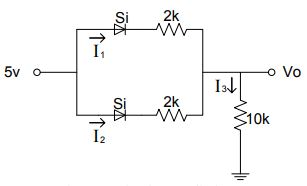
\includegraphics[scale=0.65]{fig2.JPG}

Figure 2. Diodes circuit.
\end{center}

Vivamus vitae tempus massa, vel posuere sem. Maecenas molestie mauris eu purus gravida, sit amet dignissim tortor ornare. Integer eleifend lorem libero, sit amet.

\subsection*{Diodes specifications}

Diode 1N4148:

\begin{list}
    \item {Voltage_j = 750 mV}
\end{list}
\\
\\
\\
The color-format for each resistor in Figure 2:
\begin{itemize}
    \item Resistor 1: 
    Value, value, value, value
    \item Resistor 2: 
    Value, value, value, value
    \item Resistor 3:
    Value, value, value, value
\end{itemize}
\section*{Simulating the circuit}
The code for simulate the entire circuit given in Figure 2: 

Vivamus vitae tempus massa, vel posuere sem. Maecenas molestie mauris eu purus gravida, sit amet dignissim tortor ornare. 

\begin{tabular}{|c|c|c|c|c|}
     \hline
     $V$ & $V_0$ & $I_1$(mA) & $I_2$(mA) & $I_3$(mA) \\
     \hline
     0.00 & 0.00 & 0.00 & 0.00 & 0.00 \\
     \hline
     0.00 & 0.00 & 0.00 & 0.00 & 0.00 \\
     \hline
     0.00 & 0.00 & 0.00 & 0.00 & 0.00 \\
     \hline
     0.00 & 0.00 & 0.00 & 0.00 & 0.00 \\
    \hline
    0.00 & 0.00 & 0.00 & 0.00 & 0.00 \\
    \hline
    0.00 & 0.00 & 0.00 & 0.00 & 0.00 \\
    \hline
\end{tabular}
\\
\\
\\
5. Vivamus vitae tempus massa, vel posuere sem. Maecenas molestie mauris eu purus gravida, sit amet dignissim tortor ornare.
\begin{itemize}
    \item $V_p$ = 5
    \item Offset = 0
    \item Freq = 1kHz
\end{itemize}
\begin{center}
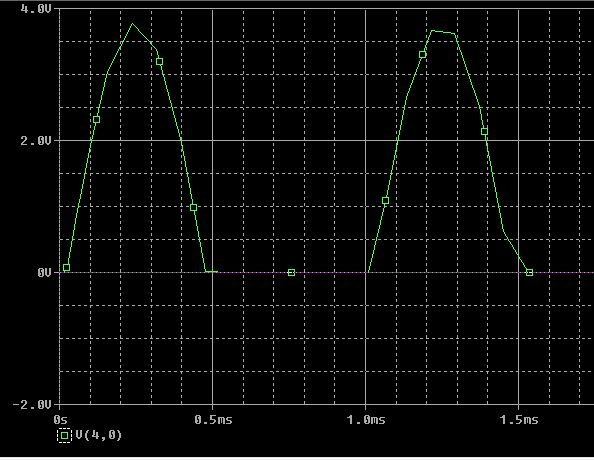
\includegraphics[scale=0.5]{elec_fig3.JPG}  Figure 3. Voltage wave.
\end{center}

\\
6. Add a capacitor in parallel with the 10k$\Omega$ resistor. \\
Lorem ipsum dolor sit amet, consectetur adipiscing elit. Sed nec turpis massa. Aliquam erat volutpat. Mauris ornare ex id augue rhoncus tincidunt: 

\begin{center}
\begin{tabular}{|c|c|}
     \hline
    Cap (uF) & Ripple Voltage (mV) \\
     \hline
     0 & 1V \\
     \hline
     0 & 1V\\
     \hline
     5 & 1V\\
     \hline
     15 & 1V\\
     \hline
     500 & 1V\\
     \hline
\end{tabular}
\end{center}

\textbf{What happened with the ripple voltage when the capacitor value increased?}\\
R: TLorem ipsum dolor sit amet, consectetur adipiscing elit. Sed nec turpis massa.\\

\textbf{Why?}\\
R: Lorem ipsum dolor sit amet, consectetur adipiscing elit. Sed nec turpis massa. Aliquam erat volutpat. Mauris ornare ex id augue rhoncus tincidunt.


\section*{Conclusion}
Lorem ipsum dolor sit amet, consectetur adipiscing elit. Sed nec turpis massa. Aliquam erat volutpat. Mauris ornare ex id augue rhoncus tincidunt:\\
Lorem ipsum dolor sit amet, consectetur adipiscing elit. Sed nec turpis massa. Aliquam erat volutpat. Mauris ornare ex id augue rhoncus tincidunt. Lorem ipsum dolor sit amet, consectetur adipiscing elit. Sed nec turpis massa. Aliquam erat volutpat. 


\section{Circuit simulation on PsPice }
\section*{Introduction}
Lorem ipsum dolor sit amet, consectetur adipiscing elit. Sed nec turpis massa. Aliquam erat volutpat. Mauris ornare ex id augue rhoncus tincidunt. Lorem ipsum dolor sit amet, consectetur adipiscing elit. Sed nec turpis massa. Aliquam erat volutpat. Mauris ornare ex id augue rhoncus tincidunt. Lorem ipsum dolor sit amet, consectetur adipiscing elit. Sed nec turpis massa. Aliquam erat volutpat. Mauris ornare ex id augue rhoncus tincidunt. 
\section*{Description}
Lorem ipsum dolor sit amet, consectetur adipiscing elit. Sed nec turpis massa. Aliquam erat volutpat. 

\begin{center}
    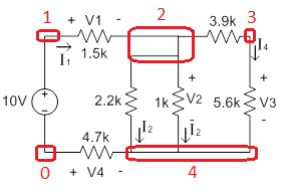
\includegraphics[scale=0.7]{fig4.JPG}
\end{center}
Lorem ipsum dolor sit amet, consectetur adipiscing elit. Sed nec turpis massa. Aliquam erat volutpat. Mauris ornare ex id:
\begin{center}
\begin{verbatim}
        Vxx = Node+ Node- Value
\end{verbatim}
\end{center}
For the voltage source, the codeline should look like the following:

\begin{verbatim}
                V1 1 0 10 V
\end{verbatim}

Lorem ipsum dolor sit amet, consectetur adipiscing elit. Sed nec turpis massa:

\begin{verbatim}
            Rxx node1 node2 VALUE
\end{verbatim}

Lorem ipsum dolor sit amet, consectetur adipiscing:

\begin{verbatim}
                R1 1 2 1.5k
\end{verbatim}

Lorem ipsum dolor sit amet, consectetur adipiscing elit. Sed nec turpis massa. Aliquam erat volutpat. Mauris ornare ex id augue rhoncus tincidunt.

\begin{verbatim}
    * CIRCUIT 1. FIGURE 3 -------------
       If (int i = 0;i<100;i+=2){
    print($"El numero actual es: {i}");
       }
       else{
    print("El bucle ya se termino");
       }
    * --------------------------------
\end{verbatim}

Lorem ipsum dolor sit amet, consectetur adipiscing elit. Sed nec turpis massa. Aliquam erat volutpat. Mauris ornare ex id augue rhoncus tincidunt. 
Lorem ipsum dolor sit amet, consectetur adipiscing elit. Sed nec turpis massa. Aliquam erat volutpat. Mauris ornare ex id augue rhoncus tincidunt. \\

\textbf{Lorem ipsum dolor sit amet, consectetur adipiscing?}

\begin{itemize}
    \item Node 1 : 33333V
    \item Node 2:  33333V
    \item Node 3:  33333V
    \item Node 4:  33333V
\end{itemize}

\textbf{Lorem ipsum dolor sit amet, consectetur adipiscing?}

R: $Total Power Dissipation = 1.46 \cdot 10^{-2} Watts$
\\
\\
\\

Lorem ipsum dolor sit amet, consectetur adipiscing elit. Sed nec turpis massa. Aliquam erat volutpat. Mauris ornare ex id augue rhoncus tincidunt.
\begin{center}
    

\begin{tabular}{|c|c|c|c|c|}
    \hline
    $V_{DC}$ (V) & I_1 (A) & I_2 (A) & I_3 (A) & I_4 (A) \\
    \hline
     1 & 0.000 & 0.000 & 0.000 & 0.000 \\
    \hline
     2 & 0.000 & 0.000 & 0.000 & 0.000 \\
    \hline
     3 & 0.000 & 0.000 & 0.000 & 0.000 \\
    \hline 
     4 & 0.000 & 0.000 & 0.000 & 0.000 \\
     \hline
     5 & 0.000 & 0.000 & 0.000 & 0.000 \\
     \hline
     6 & 0.000 & 0.000 & 0.000 & 0.000 \\
     \hline
     
\end{tabular}
\end{center}

\\
\\
\\

\section*{Conclusion}
Vivamus vitae tempus massa, vel posuere sem. Maecenas molestie mauris eu purus gravida, sit amet dignissim tortor ornare. Integer eleifend lorem libero.
\\

Vivamus vitae tempus massa, vel posuere sem. Maecenas molestie mauris eu purus gravida, sit amet dignissim tortor ornare. Integer eleifend lorem liberoVivamus vitae tempus massa, vel posuere sem. Maecenas molestie mauris eu purus gravida, sit amet dignissim tortor ornare. Integer eleifend lorem libero.
\\

Vivamus vitae tempus massa, vel posuere sem. Maecenas molestie mauris eu purus gravida, sit amet dignissim tortor ornare. Integer eleifend lorem libero. Vivamus vitae tempus massa, vel posuere sem. Maecenas molestie mauris eu purus gravida, sit amet dignissim tortor ornare. Integer eleifend lorem libero. 

\end{document}